\documentclass[11pt,a4paper]{article}
\usepackage{ngerman}
\usepackage[ngerman]{babel}
\usepackage[utf8x]{inputenc}
\usepackage[T1]{fontenc}
\usepackage{lmodern}
\usepackage{marvosym}
\usepackage{amsfonts,amsmath,amssymb}
\usepackage{textcomp}
\usepackage{pifont}
\usepackage{ifpdf}
\usepackage[pdftex]{color}
\ifpdf
  \usepackage[pdftex]{graphicx}
\else
  \usepackage[dvips]{graphicx}\fi

\pagestyle{empty}

\usepackage[scale=0.775]{geometry}
\setlength{\parindent}{0pt}
\addtolength{\parskip}{6pt}

\def\firstname{Pascal}
\def\familyname{Bernhard}
\def\FileAuthor{\firstname~\familyname}
\def\FileTitle{\firstname~\familyname's Reformation}
\def\FileSubject{Reformation}
\def\FileKeyWords{\firstname~\familyname, Reformation}

\renewcommand{\ttdefault}{pcr}
\hyphenation{ins-be-son-de-re}
\usepackage{url}
\urlstyle{tt}
\ifpdf
  \usepackage[pdftex,pdfborder=0,breaklinks,baseurl=http://,pdfpagemode=None,pdfstartview=XYZ,pdfstartpage=1]{hyperref}
  \hypersetup{
    pdfauthor   = \FileAuthor,%
    pdftitle    = \FileTitle,%
    pdfsubject  = \FileSubject,%
    pdfkeywords = \FileKeyWords,%
    pdfcreator  = \LaTeX,%
    pdfproducer = \LaTeX}
\else
  \usepackage[dvips]{hyperref}
\fi

\definecolor{firstnamecolor}{RGB}{56,115,179}
\definecolor{familynamecolor}{RGB}{56,115,179}
\hypersetup{pdfborder=0 0 0}

% Gleiche Schriftart für Hyperlinks
\urlstyle{same}


%  Gefrickel um URL-Links vernünftig umzubrechen
\makeatletter
\g@addto@macro\UrlBreaks{
  \do\a\do\b\do\c\do\d\do\e\do\f\do\g\do\h\do\i\do\j
  \do\k\do\l\do\m\do\n\do\o\do\p\do\q\do\r\do\s\do\t
  \do\u\do\v\do\w\do\x\do\y\do\z\do\&\do\1\do\2\do\3
  \do\4\do\5\do\6\do\7\do\8\do\9\do\0}
% \def\do@url@hyp{\do\-}

% Hiermit soll einer übervolle Box verhindert werden -- funktioniert sogar irgendwie
\g@addto@macro\UrlSpecials{\do\/{\mbox{\UrlFont/}\hskip 0pt plus 1pt}}
\makeatother

% Farben werden hier definiert
\definecolor{MidnightBlue}{RGB}{0,103,149}


\begin{document}
\sffamily   % for use with a résumé using sans serif fonts;
%\rmfamily  % for use with a résumé using serif fonts;
\hfill%
\begin{minipage}[t]{.6\textwidth}
\raggedleft%
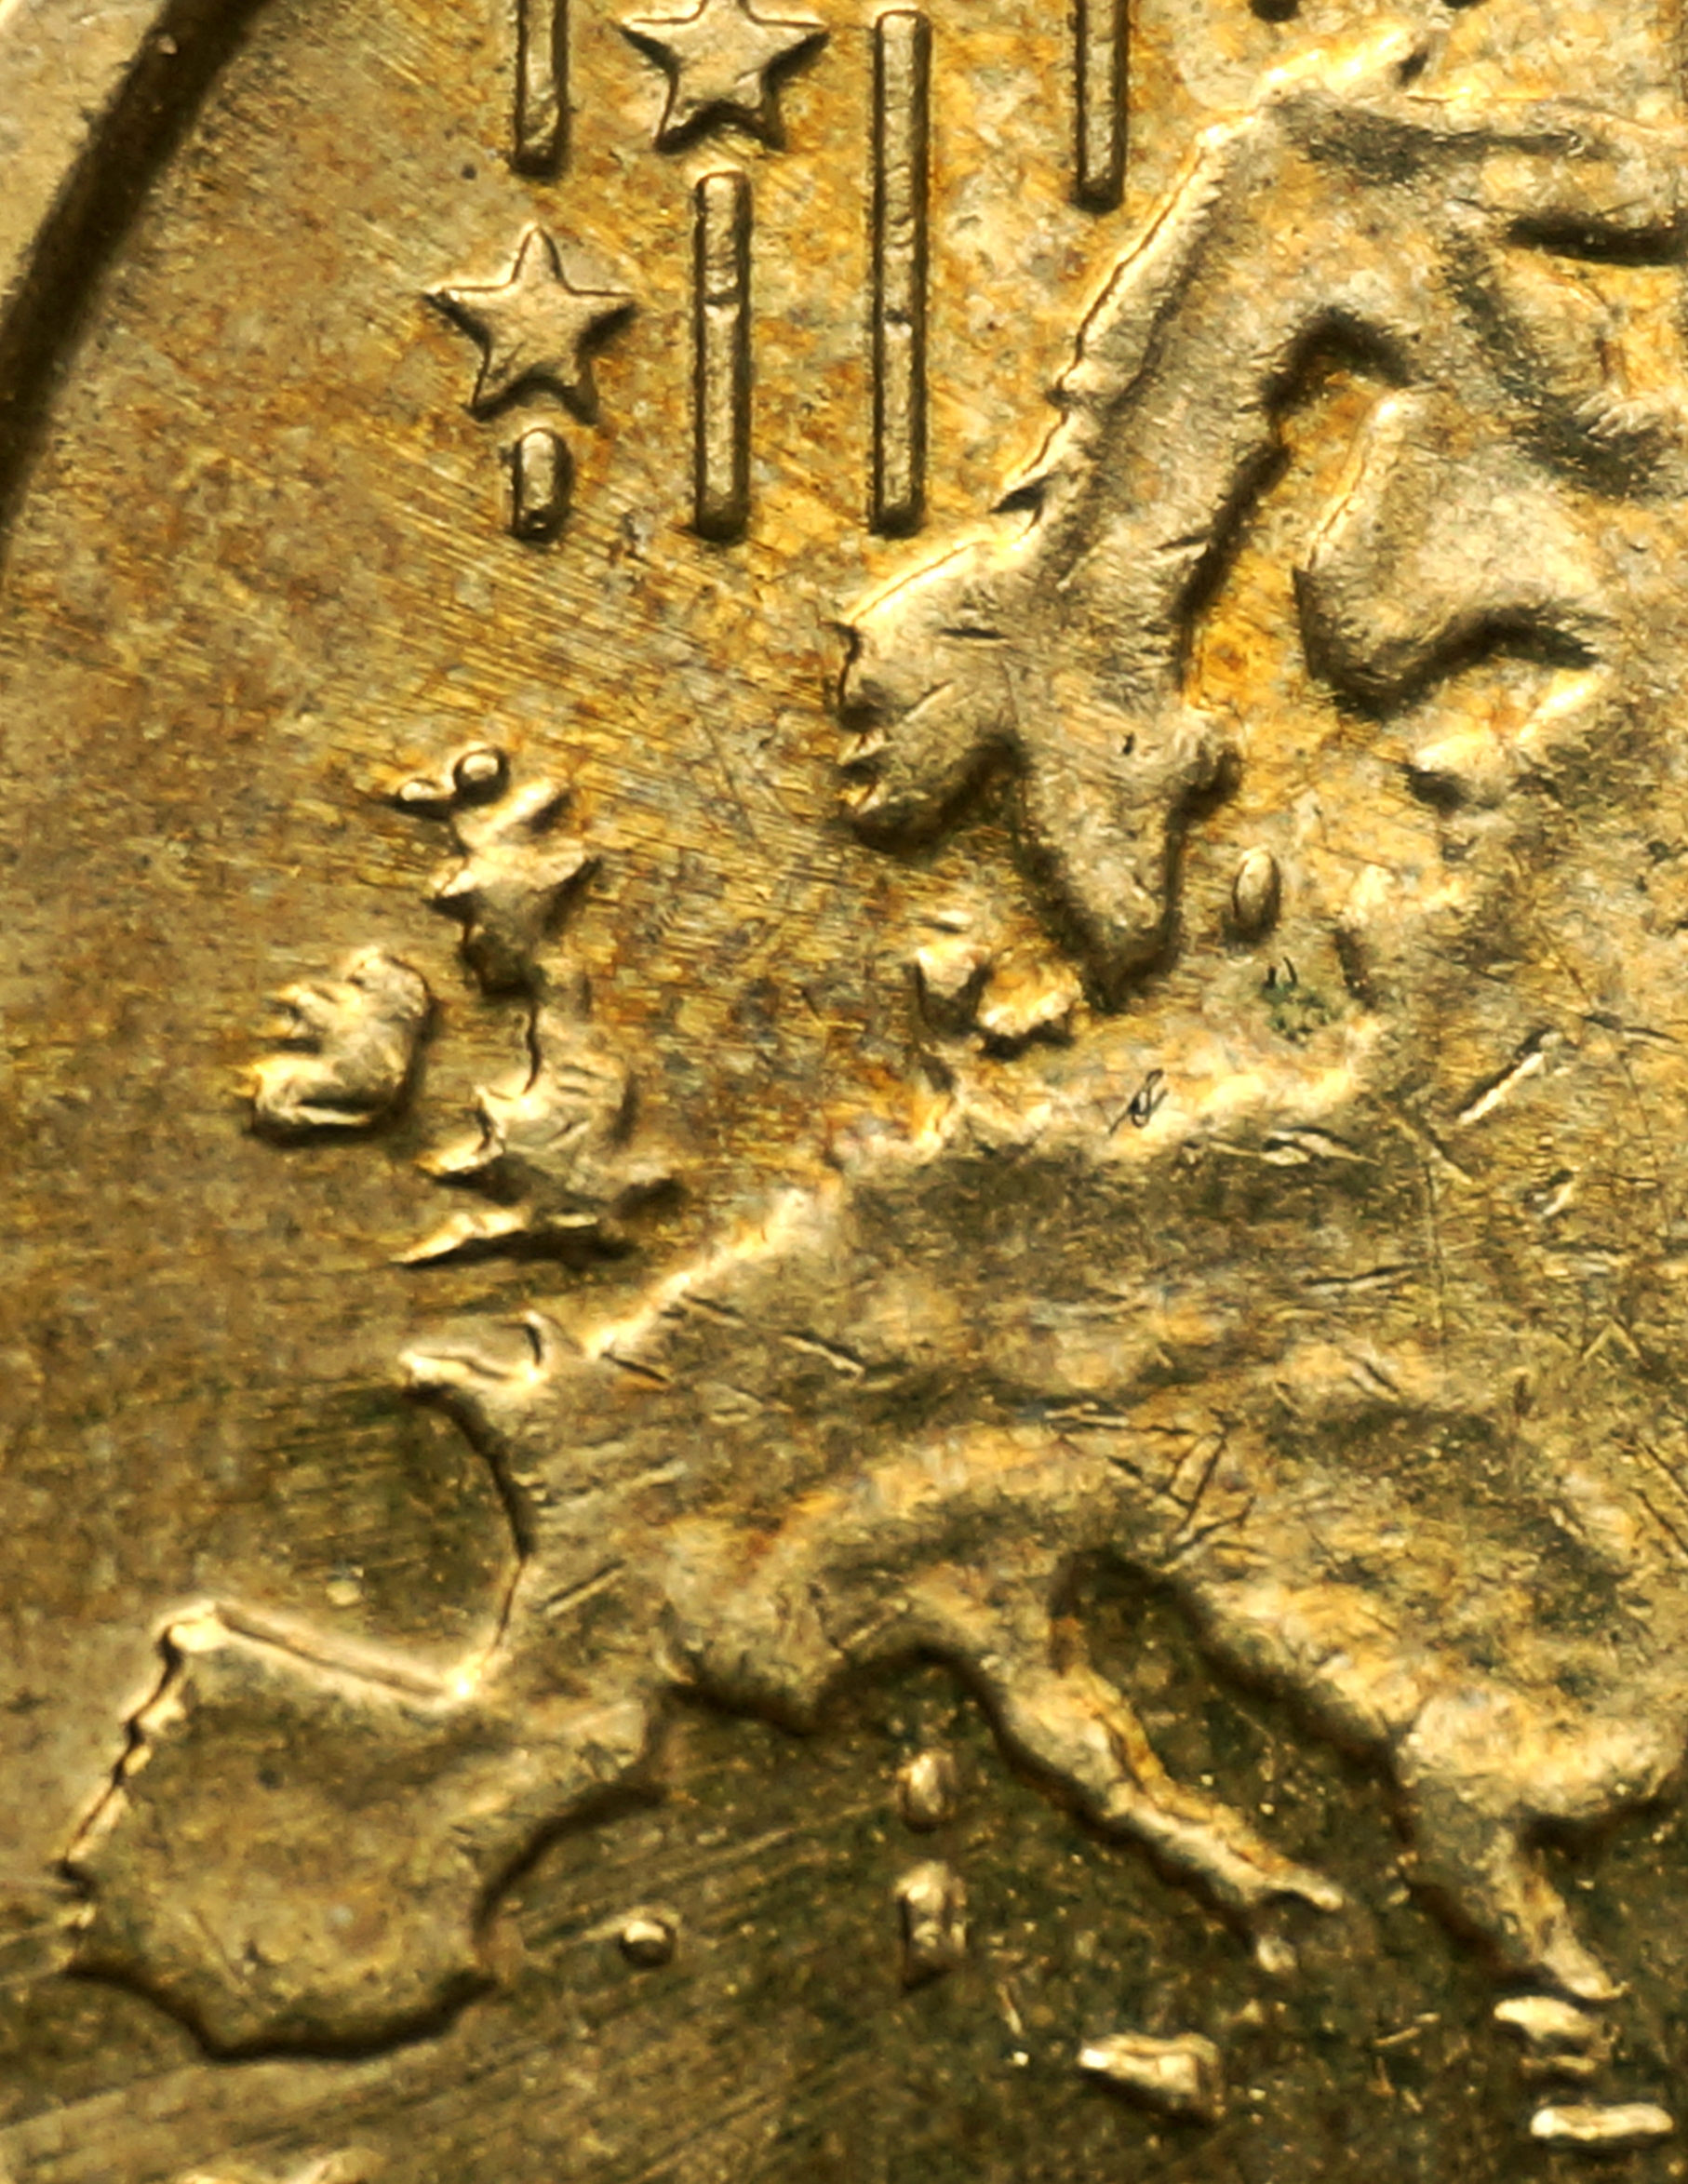
\includegraphics[width=0.55\textwidth]{Europa-auf-Muenze.jpg}


%	{\bfseries {\color{firstnamecolor}\firstname}~{\color{familynamecolor}\familyname}}\\[.35ex]
%	\small\itshape%
%	Schwalbacher Straße 7\\
%	12161 Berlin\\[.35ex]
%	\Mobilefone~+49 162 32 39 557 \\
%	\Letter~\href{mailto:pascal.bernhard@rppr.de}{pascal.bernhard@rppr.de}
\end{minipage}\\[0.5em]
%
{\color{firstnamecolor}\rule{\textwidth}{.25ex}}
%
\begin{minipage}[t]{.4\textwidth}
	\raggedright%
	% {\bfseries {\color{firstnamecolor}
	\vspace*{1em}
	\textbf{Europäische Identität} \\
%	 \\[.35ex]
	% }}
	\small%
%	Wolframstraße 89-92\\
%	12105 Berlin
\end{minipage}
%
\hfill
%
\begin{minipage}[t]{.4\textwidth}
	\raggedleft % US style
	\today
	%April 6, 2006 % US informal style
	%05/04/2006 % UK formal style
\end{minipage}\\[2.2em]


{\bfseries \color{familynamecolor}{Wurzeln der Europäischen Identität}}\\[0.75em]

\section*{\textsf{Europäische Antike und Moderne}}

\begin{itemize}
\item die Entwicklung der Kultur- und Geistesgeschichte Europas vollzog sich durch die kontinuierliche Auseinandersetzung mit antiken Errungenschaften
\item die war keine lineare Entwicklung, sondern durchlief Brüche, Missverständnisse und Umwege

	\begin{itemize}
	\item Renaissance
	\item Humanismus
	\item Klassizismus
	\item Neu-Humanismus im 19. und 20. Jahrhundert
	\end{itemize}

\item Höhere Bildung an Universitäten war auf das Studium der antiken Wissenschaften ausgerichtet

\item Kanon der \textsl{Artes liberales}: Grammatik, Rhetorik, Arithmetik, Geometrie, Musik und Astronomie wurde im Mittelalter bis in die Neuzeit als Lehrplan benutzt\\
\ding{225} antikes Wissen wurde somit weitergegeben

\end{itemize}

\subsection*{\textsf{Griechische Antike als Wiege der Europäischen Kultur}}

\begin{itemize}
\item griechische Philosophen: \textsl{Aristoteles}, \textsl{Plato}, \textsl{Stoa}\\
\ding{225} vernunftgerechtes Leben -- nicht allein Gott-gesteuert\\
\ding{225} Menschen haben Handlungsfreiheit und Verantwortung für sich selbst
\item Naturwissenschaften: \textsl{Archimedes}, \textsl{Thales von Milet}, \textsl{Pythagoras}
\item politische Philosophie: \textsl{in der griechischen Antike war die Gleichheit aller und die Beteiligung möglichst vieler Gruppen am politischen Leben eine zentrale Idee}\\
\ding{225} geistliche und weltliche Macht waren voneinander getrennt
\end{itemize}

\begin{itemize}
\item für die Griechen spielte die Unterscheidung zwischen Asien und Europa lange Zeit keine Rolle
\item erst die Bedrohung durch die Perser ließ eine Polarisierung zwischen Europa und Asien entstehen\\
\ding{225} Europa wurde mit Freiheit gleichgesetzt\\
\ding{225} mit Asien verbanden die Griechen Despotismus und Alleinherrschaft
\end{itemize}


\subsection*{\textsf{Das Römische Reich als Vorbild und Abschreckung}}

\begin{itemize}
\item das Römische Reich hatte viele Eigenschaften, welche die EU anstrebt

	\begin{enumerate}
	\item allgemeingültige Währung
	\item einheitliches Rechtssystem
	\item (phasenweise) Religionsvielfalt (von den Christenverfolgungen abgesehen)
	\item friedliche Grenzen -- keine Bedrohung von Außen
	\item gemeinsame Sprache
	\item erstrebenswerte Zivilisation
	\end{enumerate}

\item das Römische Reiche hatte einen erheblichen Anteil an der Formierung des politischen und kulturellen Europas in Mittelalter und Neuzeit


	\begin{itemize}
	\item Ausbreitung des Christentums
	\item Etablierung einer Staatsreligion
	\item Latein als Sprache und Mittel zur Bewahrung der Kultur wurde ins Mittelalter übertragen
	\item Latein war bis in die Moderne das einende Element der Europäischen Elite und Kultur
	\end{itemize}

\item römisches Recht bildet Grundlage der Entwicklung moderner europäischer Rechtssysteme

	\begin{itemize}
	\item aus Recht wurde Gesetz
	\ding{225} ohne Gesetz gab es kein Recht (\textsl{sine lege nulla poena})
	\item Recht war niedergeschrieben und nicht willkürlich durch Könige oder Priester ausgeteilt
	\item römisches Recht war auf Lebenspraxis der Bürger und Bedürfnisse nach Gerechtigkeit ausgerichtet
	\end{itemize}

\item durch den Aufstieg der katholischen Kirche trat das kanonische Recht zunehmend gleichberechtigt an die Seite des römischen Rechts

\item in Frankreich, Deutschland und England wurde das auf römischem Rechts basierende System durch Gewohnheitsrecht ergänzt

\item im Zuge der Aufklärung und dem Aufkommen der Idee von Menschenrechten gewann das System logischer Schlussfolgerungen und auf Vernunft basierender Gesetze erneut an Bedeutung

\subsection*{\textsf{Wichtige Ideen antiken Ursprungs:}}


\begin{itemize}
\item Glaube an eine übernationale Ordnung
\item Innerer und Äußerer Frieden
\item Rechtsgleichheit
\item Würde und Autonomie des Einzelnen
\item Trennung von geistlicher und weltlicher Macht
\end{itemize}


\end{itemize}


\end{document}